\begin{figure}[ht!]
\centering
\subfigure[$A$]
{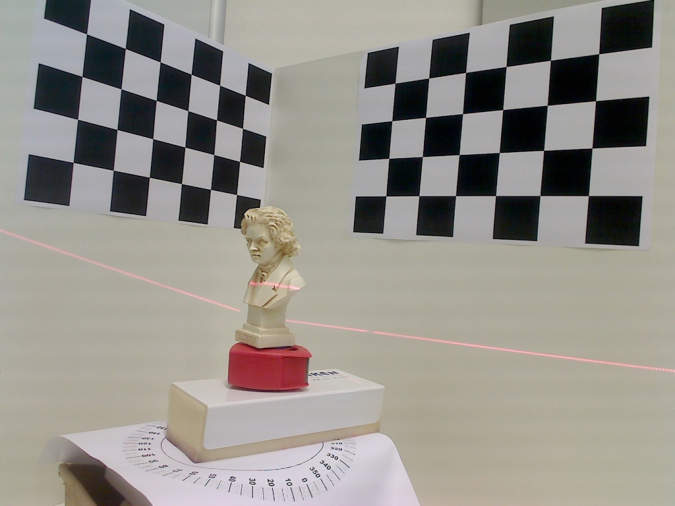
\includegraphics[width=.45\linewidth]{figures/difference-1}
 \label{subfigure:diff-A}} \hfill
\subfigure[$B$]
{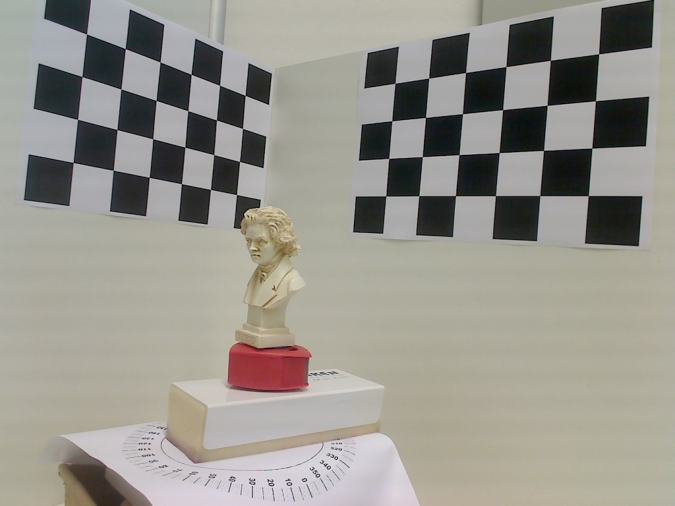
\includegraphics[width=.45\linewidth]{figures/difference-2}
\label{subfigure:diff-B}} \\
\subfigure[$C$]
{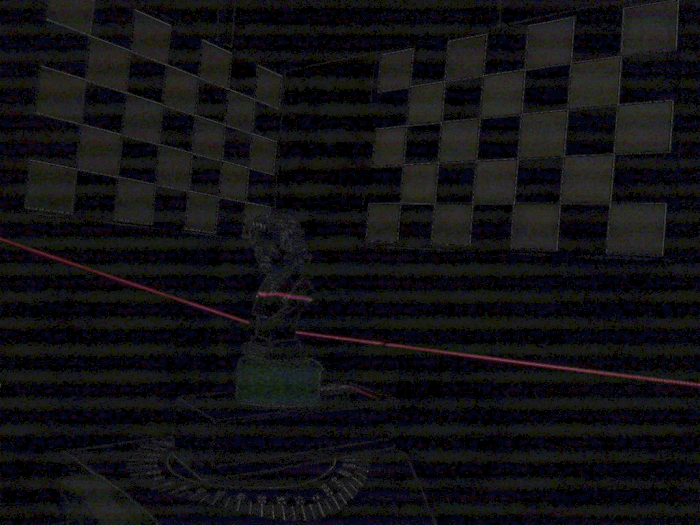
\includegraphics[width=.45\linewidth]{figures/difference-3}
\label{subfigure:diff-C}} \hfill
\caption{Using Image Difference to Find the Laser}
\label{figure:difference-image}
\end{figure}

We used OpenCV routine \texttt{cvAbsDiff()} to calculate the image difference
of the laser image from the reference image using equation
\ref{equation:difference-image}. The resulted image difference is shown in
Fig. \ref{figure:difference-image}

\begin{align}
\label{equation:difference-image}
C = A &- B \\
\text{where}~
&A~ \text{is the laser image in figure \ref{subfigure:diff-A} and} \notag \\
&B~ \text{is the reference image in figure \ref{subfigure:diff-B} and} \notag \\
&C~ \text{is the difference image in figure \ref{subfigure:diff-C}} \notag
\end{align}

To reduce the noise in the difference image, we used the OpenCV
routine \texttt{cvSmooth()} to convolve the image with a Gaussian kernel
function as shown in Fig. \ref{figure:gauss}. It not only helped us to
remove the camera artifacts but also reduce the information content in the
image.

\begin{figure}[ht!]
\centering
\subfigure[Difference Image]
{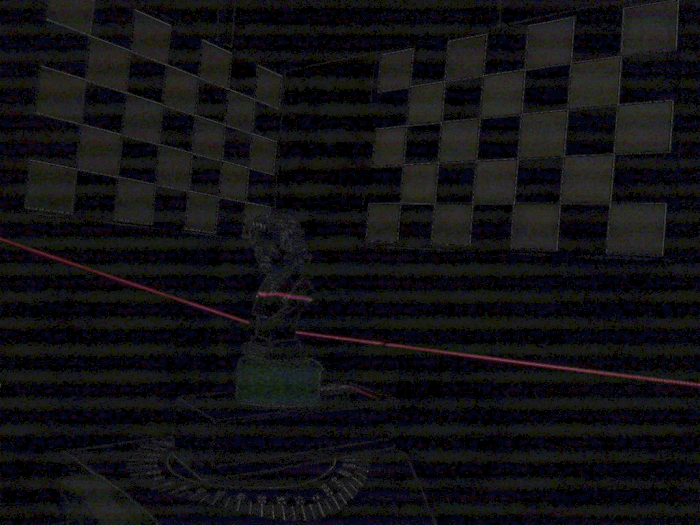
\includegraphics[width=.45\linewidth]{figures/difference-3}
\label{subfigure:gauss-A}} \quad
\subfigure[Gaussian Smoothened Image]
{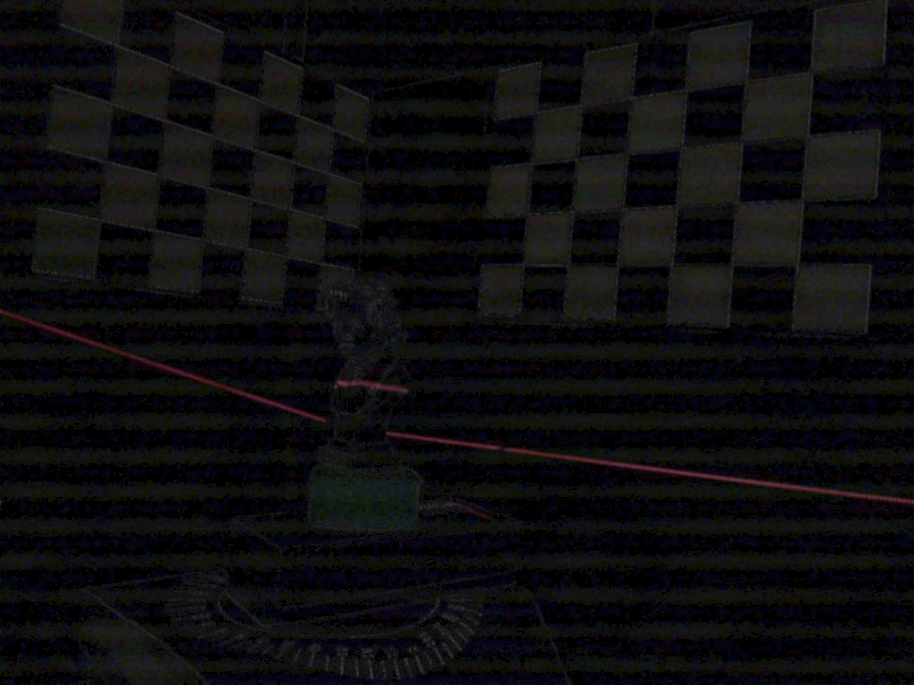
\includegraphics[width=.45\linewidth]{figures/gauss}
\label{subfigure:gauss-B}} \hfill
\caption{Gaussian Smoothing the Difference Image}
\label{figure:gauss}
\end{figure}

In order to remove all outliers and keep just the pixels
representing the red laser line as shown in Fig. \ref{figure:color-thres},
we used a pre-defined threshold value for the intensity of the red pixels. In
order to restrict this thresholding only along the red channel, we used
\texttt{cvSplit()} to split the three-channel (R,G,B) difference image into
separate one-channel image planes. We used \texttt{cvGet2D()} and
\texttt{cvSet2D()} to work on the scalar intensity values of the pixels.

\begin{figure}[ht!]
\centering
\subfigure[Image with Outliers]
{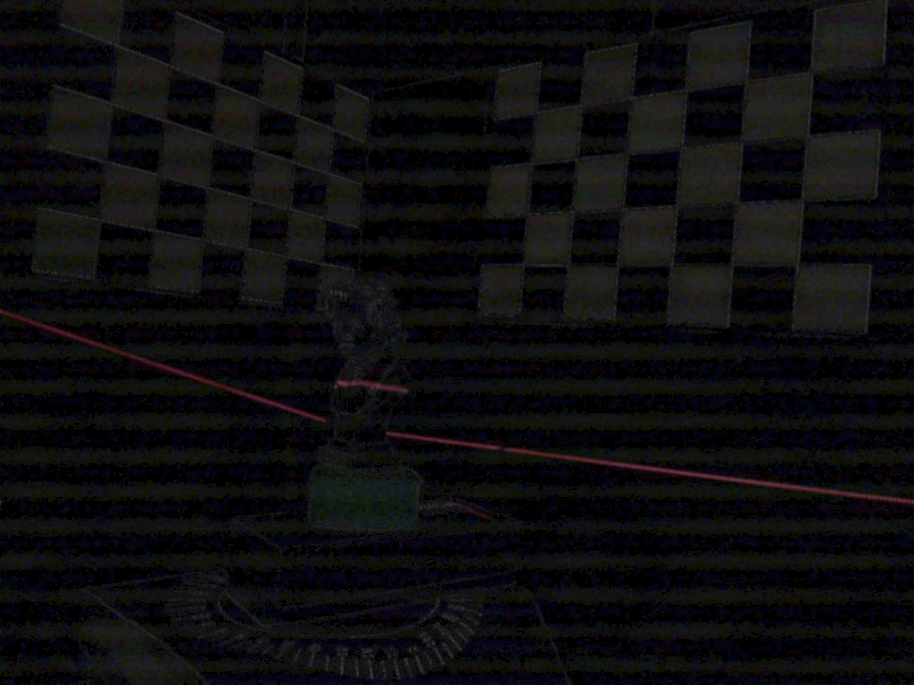
\includegraphics[width=.45\linewidth]{figures/gauss}
\label{subfigure:colorthres-A}} \quad
\subfigure[Image without Outliers]
{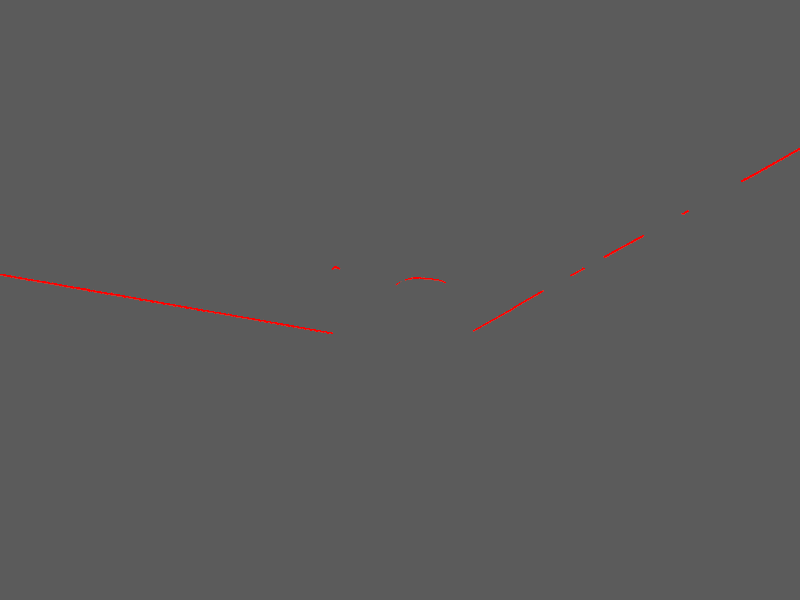
\includegraphics[width=.45\linewidth]{figures/colorthres}
\label{subfigure:colorthres-B}} \hfill
\caption{Color Thresholding to Remove Outliers}
\label{figure:color-thres}
\end{figure}

We use \ac{PPHT} \cite{kiryati:1991}, \cite{matas:2000} using OpenCV routine
\texttt{cvHoughLines2()} to detect the laser lines on both sides of the target
object. The line end points of each line thus obtained were used to draw the
line using \texttt{cvLine()} as shown in Fig. \ref{figure:hough-transform}.
The difference image was initially passed through an edge detection phase,
since hough transform not only expects a gray-scale image as input but the
input is also treated as binary information where the non-zero points are edge
points of the image. Therefore, we used OpenCV routine \texttt{cvCvtColor} to
convert the RGB difference image to gray scale and \texttt{cvCanny()} to
perform the Canny Edge Detection \cite{canny:1986} before \ac{PPHT}. The two
hough line equations on either side of the object were used to learn the laser
line points, while the points not identified as part of the hough line were
taken as target object points.

\begin{figure}[ht!]
\centering
\subfigure[Before Transformation]
{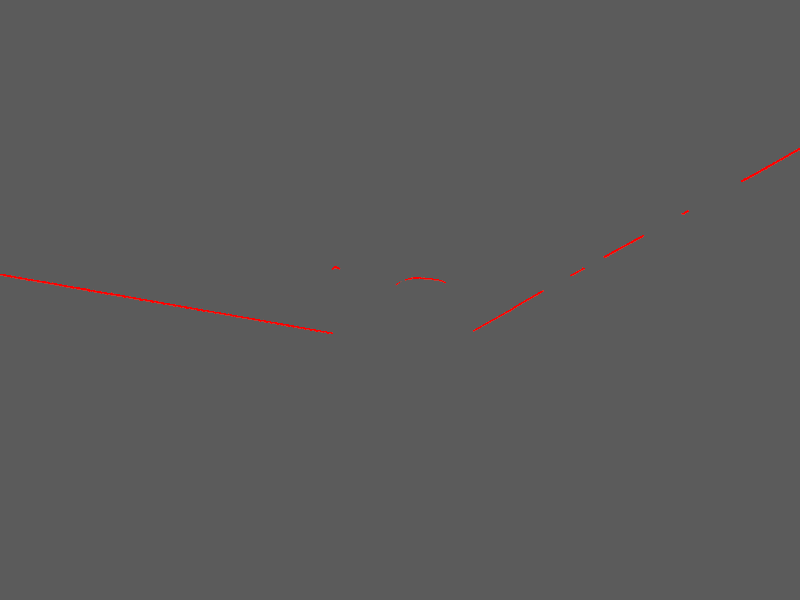
\includegraphics[width=.45\linewidth]{figures/colorthres}
\label{subfigure:hough-A}} \quad
\subfigure[After Transformation]
{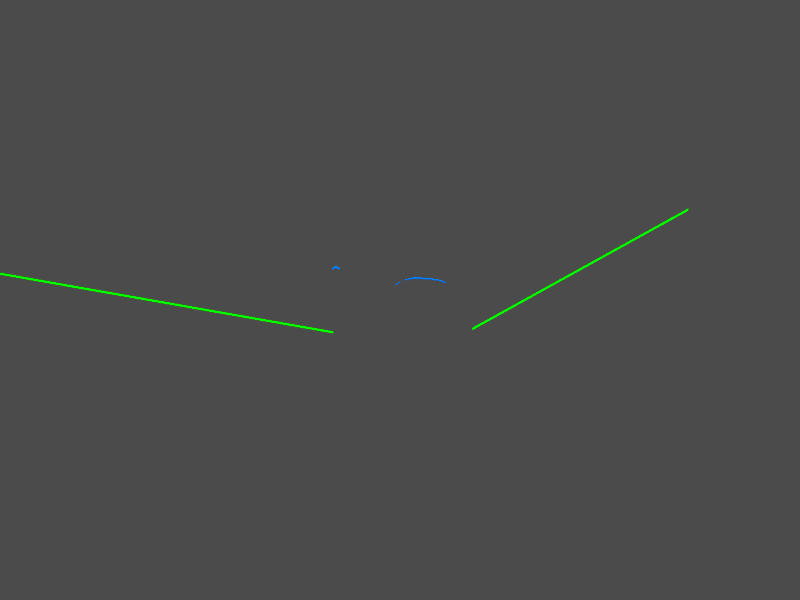
\includegraphics[width=.45\linewidth]{figures/hough}
\label{subfigure:hough-B}} \hfill
\caption{Hough Transformation}
\label{figure:hough-transform}
\end{figure}
